\documentclass{article}
\usepackage{custom} %% Have stripped out journal/publisher identifiers and trim marks
% \usepackage{maa-monthly} %% For actual journal style
\usepackage{textcomp}

\usepackage{algorithm2e}

%% IF YOU HAVE FONTS INSTALLED
%\usepackage{mtpro2}
%\usepackage{mathtime}
\usepackage{amsfonts}

\theoremstyle{plain}
\newtheorem{theorem}{Theorem}
\newtheorem{lemma}{Lemma}
 
\theoremstyle{definition}
\newtheorem*{definition}{Definition}
\newtheorem*{remark}{Remark}
\newtheorem{example}{Example}

\def \cC {\mathcal{C}}
\def \cG {\mathcal{G}}
\def \cP {\mathcal{P}}
\def \FF {\mathbb{F}}
\newcommand{\AND}{\mathbin{\texttt{\&}}}
\DeclareMathOperator{\im}{im}
\def\And{\mathbin{\&}}
\def\Plus{+}
\DeclareMathOperator{\Span}{span}
\DeclareMathOperator{\Length}{length}

\begin{document}

\title{(Re)constructing code loops}
\markright{Reconstructing code loops}
\author{Ben Nagy and David Michael Roberts}

\maketitle

\begin{abstract}
Write later.
\end{abstract}


\noindent
The theory of codes makes for a fascinating study. 
At their heart, codes are `merely' subspaces of vector spaces over some small finite field, with certain combinatorial properties.
Why do such things exist? Like a lot of exceptional objects in combinatorics, it can come down to: ``because''.
This makes constructing codes sometimes more of an art than something systematic.
In this paper, we are going to consider the construction of certain structures closely related to codes, called \emph{code loops}. 
We will also only be considering the case where the base field is $\FF_2=\{0,1\}$, and refer to its elements as \emph{bits}.

The first published example of a code loop appeared as a step in John Conway's construction of the Monster sporadic simple group \cite{Conway}. 
The code loop Conway used originally appeared in an unpublished manuscript by Richard Parker.
A general study of code loops was then made by Robert Griess \cite{Griess}.
Griess also proved the existence of code loops by an algorithmic construction, starting from a particular type of code.
More recent approaches will be discussed below.

Recall that the elements (or \emph{words}) in a code $\cC$, being vectors, can be combined by addition---this is a group operation and hence associative. 
The elements of a code loop consist of a pair: a code word and one extra bit.
The extra bit \emph{twists} the addition so that combination of code loop elements is a \emph{non-associative operation}: $(xy)z\not=x(yz)$.

More specifically, while addition of words in a code is performed by co\"ordinatewise addition in $\FF_2$---bitwise XOR---the algebraic operation in a code loop is not so easily described.
The code loop operation can be reconstructed from a function $\cC \times \cC \to \FF_2$ satisfying certain identities, called a \emph{twisted cocycle}.
It is the computation and presentation of this function that will mainly concern us in this article, using Griess's algorithm \cite[proof of Theorem 10]{Griess}.
As a result, we will observe some curious features of the Parker loop, obtained via experimentation and, it seems, previously unknown.

\section{Extensions and cocycles.}

As a warm-up, we will describe a more familiar structure using the techniques that will be used later. 
Recall that the \emph{quaternion group} $Q_8$ is the group consisting of the positive and negative basis quaternions:
\[
	Q_8 = \{1,\, i,\, j,\, k,\,-1,\, -i,\, -j,\, -k\}
\]
The elements of $Q_8$ satisfy the identities
\[
	i^2 = j^2 = k^2 = -1, \quad ij=k.
\]
There is a surjective group homomorphism $\pi\colon Q_8 \to \FF_2 \times \FF_2 = V_4$, sending $i$ to $(1,0)$ and $j$ to $(0,1)$, and the kernel of $\pi$ is the subgroup $\{1,-1\}\simeq \FF_2$.
Moreover, this kernel is the \emph{center} of $Q_8$, the set of all elements that commute with every other element of the group.

Now $Q_8$ is a nonabelian group, but both $\FF_2$ and $V_4$ are abelian groups.
One might think that it shouldn't be possible to reconstruct $Q_8$ from the latter two groups, but it is! 
That is, if we are given some extra information that uses only the two abelian groups.
There is an obvious function $s\colon V_4 \to Q_8$, sending $(0,0)$ to $1$, $(1,0)$ to $i$, $(0,1)$ to $j$ and $(1,1)$ to $k$.
This almost looks like a group homomorphism, but it is not, as $(1,0) + (1,0) = (0,0)$ in $V$, but $i^2 \not= 1$ in $Q_8$.
We can measure the failure of $s$ to be a group homomorphism by considering the two-variable function
\[
	d\colon V_4 \times V_4 \to \FF_2
\]
defined by $ (-1)^{d(v,w)} = s(v)s(w)s(v+w)^{-1}$. 
It is a nice exercise to see that $s(v)s(w)s(v+w)^{-1}$ is always $\pm 1$, so that this definition makes sense. The values of $d(v,w)$ are given as:

% \medskip
\begin{center}
\begin{tabular*}{0.35\textwidth}{c|cccc}
$v\setminus w$&$00$&$10$&$01$&$11$\\
\hline
	$00$		& $0$& $0$& $0$& $0$\\
	$10$		& $0$& $1$& $1$& $0$\\
	$01$		& $0$& $0$& $1$& $1$\\
	$11$		& $0$& $1$& $0$& $1$\\
\end{tabular*}
\end{center}
where $00=(0,1)$, $10=(1,0)$ etc.
If $s$ \emph{were} a homomorphism, $d$ would be constant at $0$.
One can check that $d$ satisfies the \emph{cocycle identities}:
\[
	d(v,w)-d(u+v,w)+d(u,v+w)-d(u,v) = 0
\]
for all triples $u,v,w\in V_4$. It is also immediate from the definition that $d(0,0)=0$.
An alternative visualisation is given in Figure~\ref{fig:cocycle for q8}.

\begin{figure}[!b]
% \begin{minipage}[b]{4cm}
% \[
% \begin{array}{c|cccc}
% v\setminus w&00&10&01&11\\
% \hline
% 	00		& 0& 0& 0& 0\\
% 	10		& 0& 1& 1& 0\\
% 	01		& 0& 0& 1& 1\\
% 	11		& 0& 1& 0& 1\\
% \end{array}
% \]
% \end{minipage} 
% \hspace{1cm}
% \begin{tabular*}{0.35\textwidth}{c|cccc}
% $v\setminus w$&00&10&01&11\\
% \hline
% 	00		& 0& 0& 0& 0\\
% 	10		& 0& 1& 1& 0\\
% 	01		& 0& 0& 1& 1\\
% 	11		& 0& 1& 0& 1\\
% \end{tabular*}
% \hspace{3cm} 
\begin{center}
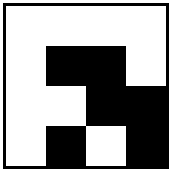
\includegraphics[height=2.5cm]{quaternion_cocyc} %%% Want this to be a pdf image, not png
\end{center}
\caption{A $4\times4$ array giving the values of the cocycle $d\colon V_4\times V_4\to \FF_2$, with white = $0$, black = $1$.}
\label{fig:cocycle for q8}
\end{figure}


The reason for this somewhat mysterious construction is that we can build a bijection of sets using $s$ and the isomorphism $\FF_2\simeq \{1,-1\}$, namely
\[
	\FF_2\times V_4 \simeq \left(\{1\}\times V_4\right) \cup \left(\{-1\} \times V_4\right) \stackrel{\phi}{\longrightarrow}
	\{1,\, i,\, j,\, k\}\cup \{-1,\, -i,\, -j,\, -k\} = Q_8
\]
If we define a new product operation on the underlying \emph{set} of $\FF_2\times V_4$ by
\[
	(s,v)\ast_d(t,w):=(s+ t+ d(v,w),v+w),
\]
then the cocycle identities ensure that this is in fact associative and further, a group operation.
Finally, $\phi$ can be checked to be a homomorphism for the group operation on $Q_8$ and for $\ast_d$, hence is a group isomorphism.

Thus we can reconstruct, at least up to isomorphism, the nonabelian group $Q_8$ from the two abelian groups $V_4$ and $\FF_2$, together with the \emph{cocycle} $d\colon V_4\times V_4\to \FF_2$.
% A table of the values of $d$ is shown in Figure~\ref{fig:cocycle for q8}, where $00=(0,0)$, $10 = (1,0)$ etc.
If we didn't know about the group structure of $Q_8$ already we could construct it from scratch using $d$.
This is what we aim to do to construct the Parker loop, using a similar approach.


\section{Twisted cocycles and loops.}

The construction in the previous section is a fairly typical case of reconstructing a central extension from a cocycle (although in general one does not even need the analogue of the group $V_4$ to be abelian). 
However, we wish to go one step further, and construct a structure with a \emph{non-associative} product from a pair of abelian groups: the group $\FF_2$ and a vector space $V$.
Instead of a cocycle, we use a \emph{twisted cocycle}: a function $\alpha\colon V\times V \to \FF_2$ like $d$ that instead satisfies
\[
	\alpha(v,w)-\alpha(u+v,w)+\alpha(u,v+w)-\alpha(u,v) = f(u,v,w),
\]
for a special \emph{twisting function} $f\colon V\times V\times V \to \FF_2$. We will assume that $\alpha$ satisfies $\alpha(0,v)=\alpha(v,0) = 0$ for all $v\in V$, a property that holds for $d$ in the previous section. From a twisted cocycle the set $\FF \times V$ can be given a binary operation
\[
	(s,v)\ast_\alpha(t,w):=(s+ t+ \alpha(v,w),v+w).
\]
We denote $\FF \times V$ equipped with this binary operation by $\FF_2\times_\alpha V$.

Recall that a \emph{loop} is a set $L$ with a binary operation $\star\colon L\times L \to L$, a unit element $e\in L$ such that $e\star x = x \star e = x$ for all $x\in L$, and such that the functions $(-)\star z \colon L \to L$ and $z\star (-) \colon L \to L$ are bijections for every $z\in L$. 
Informally, this means that every element $z\in L$ has a left inverse and a right inverse for $\star$, and these are unique---but may be different in general. 
The following is a cute exercise is using the twisting function and the assumption that $\alpha(0,v)=\alpha(v,0)=0$.

\begin{lemma}
The operation $\ast_\alpha$ makes $\FF_2\times_\alpha V$ into a loop, with identity element $(0,\underline{0})$, for $\underline{0}$ the zero vector in $V$.
\end{lemma}

Groups are examples of loops, but they are in a sense the uninteresting case. 
Arbitrary loops are quite badly behaved: their product is non-associative in general. 
But there is a special non-associative case, introduced by Ruth Moufang \cite{Moufang}, where one has better algebraic properties.

\begin{definition}
A \emph{Moufang loop} is a loop $(L,\star)$ satisfying the identity $x \star (y \star (x \star z)) = ((x \star y) \star x) \star z$ for all choices of elements $x,y,z\in L$.
\end{definition}

The most famous example of a Moufang loop is probably the non-zero octonions $\mathbb{O}^\times$ under multiplication. 
A key property of a Moufang loop $L$ is that any subloop $\langle x,y\rangle < L$ generated by a pair of elements $x,y$ is in fact a group. 
As a corollary, powers of a \emph{single} element are well-defined, and do not require extra bracketing: $x\star (x \star x) = (x\star x) \star x =: x^3$, for example. 
Additionally, the left and right inverses \emph{always} agree in a Moufang loop, so that for each $x\in L$, there is a unique $x^{-1}$ such that $x\star x^{-1} = x^{-1}\star x = e$. 
Importantly for us, code loops, defined below as a special case of the construction of $\FF\times_\alpha V$, turn out to be Moufang.

\begin{example}\label{example:m16}
The finite Moufang loop $M := M_{16}(C_2\times C_4)$ of \cite{} (classification paper, ?Moufang Loops of Small Order. I?), with 16 elements, is an extension $\FF_2 \to M \to V=\FF_2^3$ arising from a twisted cocycle $V\times V\to \FF_2$ given by the $8\times 8$ array
\medskip
\begin{center}
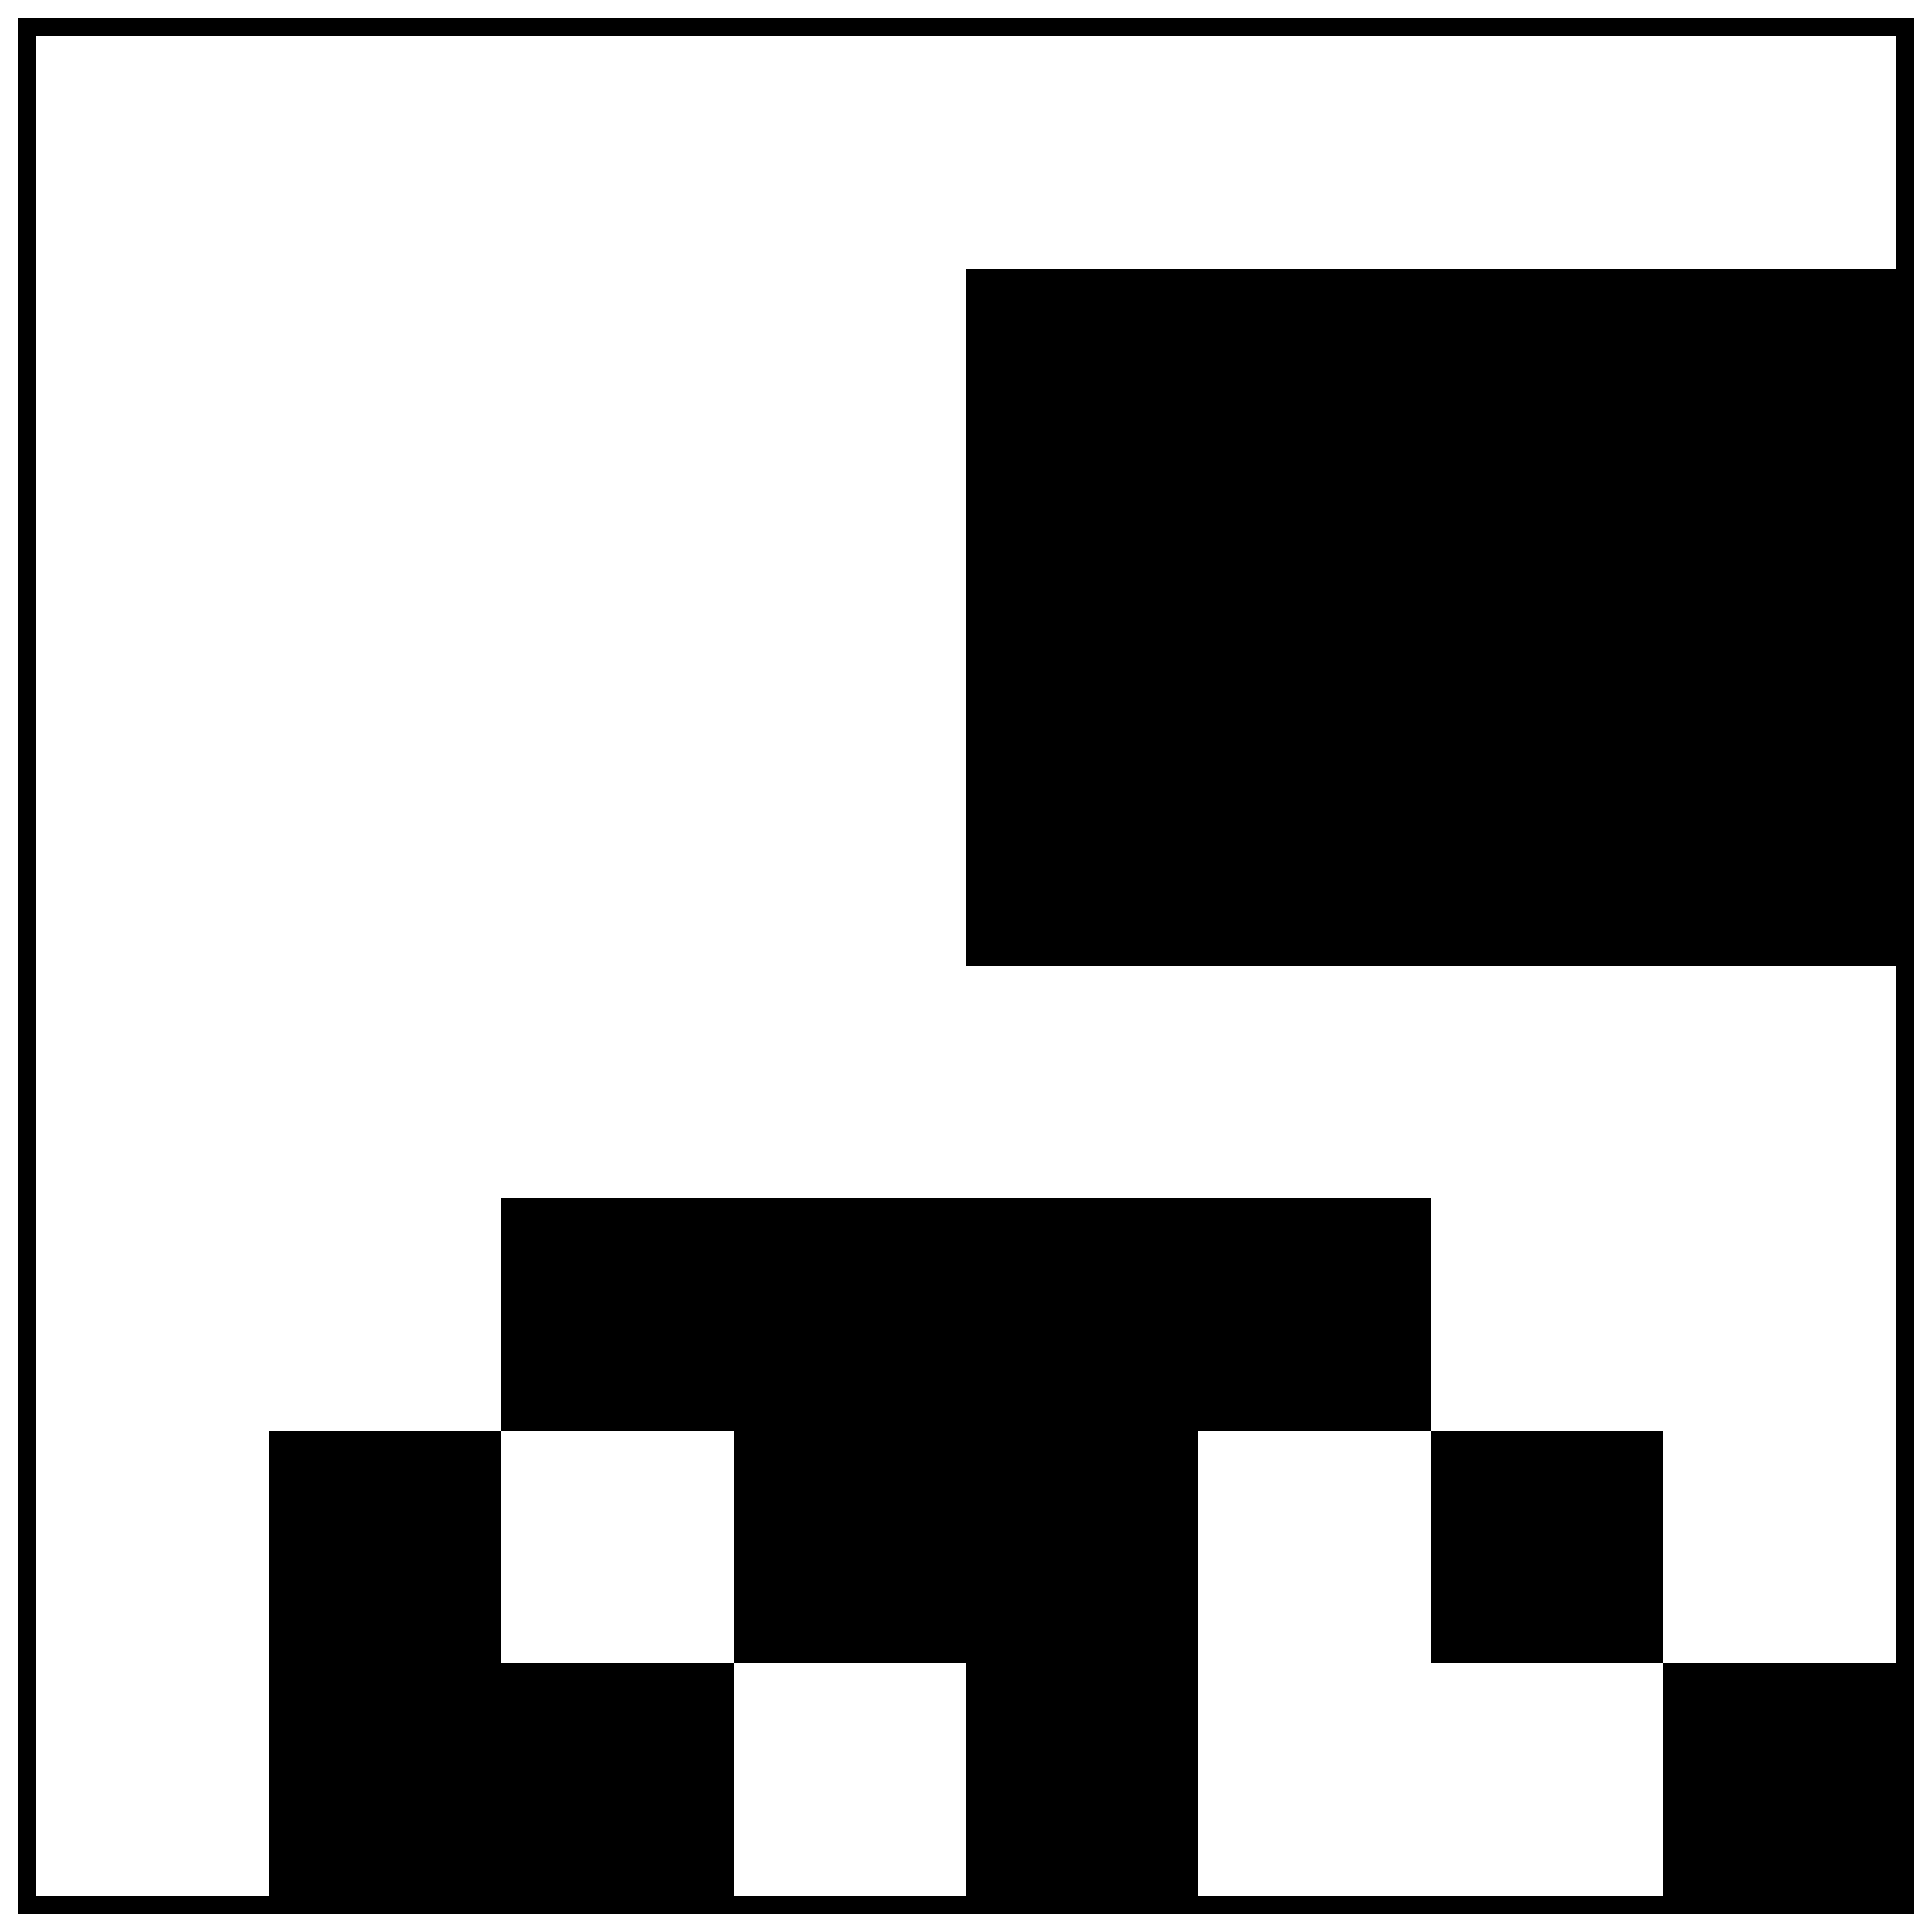
\includegraphics[width=0.25\textwidth]{m16.png}
\end{center}
where again, white = $0$, black = $1$. The order of the row/colum labels is $000$, $100$, $010$, $110$, $001$, $101$, $011$, $111$. 
Notice in particular that the first four columns/rows correspond to the subspace $U\subset V$ spanned by $10$ and $01$, and that the restriction $U\times U \to \FF_2$ is identically zero (i.e.\ white). 
This means that the restriction of $M$ to the subspace $U$---the subloop of elements that map to elements of $U$---is in fact the direct product $\FF_2\times U$, and in particular a group.
\end{example}


\section{Codes and code loops.}

To describe the twisting function $f$ for our code loops, we need to know about some extra operations that exist on vector spaces over the field $\FF_2$. 
For $W$ an $n$-dimensional vector space over $\FF_2$ and vectors $v,w\in W$, there is a new vector $v\AND w \in W$ given by
\[
	v\AND w := (v_1w_1,\,v_2w_2,\,\ldots,\,v_nw_n).
\]
If we think of such vectors as binary words, then this is bitwise AND.
Note that if we take a code $\cC \subset (\FF_2)^n$, then $\cC$ is not guaranteed to be closed under this operation.
The other operation takes a vector $v\in W$ and returns its \emph{weight}: the sum, as an integer, of its entries: $|v| := v_1 + \cdots + v_n$. 
Equivalently, it is the number of nonzero entries in $v$.

The desired twisting function is a combination of these two, namely $f(u,v,w) := |u\AND v\AND w|$.
However, as alluded to above, we also are going to ask that further identities hold. 
For these identities to make sense we need to start with a code with the special property of being \emph{doubly even}.

\begin{definition}
A code $\cC \subset (\FF_2)^n$ is \emph{doubly even} if for every word $v\in \cC$, $|v|$ is divisible by 4. 
\end{definition}


\begin{example}\label{example:Hamming}
The \emph{Hamming (8,4) code} is doubly even, and is given by the subspace of $\FF_2^8$ spanned by the rows of the matrix
\[
\begingroup % keep the change local
\setlength\arraycolsep{2pt}
\begin{pmatrix}
1&0&0&0&0&1&1&1\\
0&1&0&0&1&0&1&1\\
0&0&1&0&1&1&0&1\\
0&0&0&1&1&1&1&0
\end{pmatrix}
\endgroup
\]
\end{example}

A more substantial example is given by the Golay code.

\begin{example}\label{example:Golay}
The Golay code $\cG \subset \FF_2^{24}$ is the span of the 12 rows in the following two matrices
\[	
	 \left(\begin{array}{c}
     000110000000010110100011 \\
     101001111101101111110001 \\
     000100000000100100111110 \\
     010000000010000110101101 \\
     000000000010010101010111 \\
     100000000000100111110001
     \end{array}\right)
\qquad
    \left(\begin{array}{c}
	 101001011100111001111111 \\
	 100000011100001001001100 \\
	 000001000000111001001110 \\
	 100000001000111000111000 \\
	 100000000100101000010111 \\
	 011011000001111011111111
	 \end{array}\right)
\]
This is a different basis from the usual one \cite{Thompson}, which can be built using the complement of the incidence matrix of the icosahedron. 
This basis, however, allows us to demonstrate some interesting properties below.
\end{example}

The inclusion/exclusion formula applied to counting nonzero entries allows us to show that, for all $v$ and $w$ in any doubly even code $\cC$,
\[
	|v+w| + |v\AND w| = |v| + |w| - |v\AND w|\,.
\]
In other words: $|v\AND w| = \frac12(|v| + |w| - |v+w|)$, which implies that $|v\AND w|$ is divisible by 2.
Thus for words $v,w$ in a doubly even code, both $\frac14|v|$ and $\frac12|v\AND w|$ are integers.

\begin{definition}[Griess \cite{Griess}]
Let $\cC$ be a doubly even code. 
A \emph{code cocycle} $\alpha\colon \cC \times \cC \to \FF_2$ is a  function satisfy the identities
\begin{align}
& \alpha(v,w)-\alpha(u+v,w)+\alpha(u,v+w)-\alpha(u,v) =|u\AND v \AND w| \pmod 2 \label{eq: code cocycle 1}\\
& \alpha(v,w)+\alpha(w,v) = {}  \tfrac12|v\AND w| \pmod 2 \label{eq: code cocycle 2}\\
& \alpha(v,v) = {}  \tfrac14|v| \pmod 2\label{eq: code cocycle 3}
\end{align}
\end{definition}

\begin{remark}
What we call a code cocycle, Griess actually calls a `factor set'. Given that a code cocycle is an example of a twisted cocycle, we prefer a name that indicates this.
\end{remark}

It is not obvious, on first consideration, that code cocycles even exist, or how many there are for a given doubly even code. 
However, Griess gave an proof that inductively constructs code cocycles, and counts how many arbitrary choices can be made along the way, proving that code cocycles do indeed exist.
The growth of the number of possible code cocycles with $\dim \cC$ is rather fearsome: $2^{2^k-k-1}$, for $k=\dim \cC$ (\cite[Theorem 10]{Griess}).
For the 4-dimensional Hamming code given above, this is $512$, but for the extended Golay code below there are $2^{4083}$ possible code cocycles, a number with $1230$ digits in base $10$.



\section{Griess's algorithm and its output.}

The algorithm that Griess gives in \cite[Theorem 10]{Griess} to construct code cocycles for a code $\cC$ takes as input an ordered  basis $\{b_1,\ldots,b_k\}$ for $\cC$. 
The code cocycle is then built up inductively over larger and larger subspaces $\Span\{b_1,\ldots,b_m\}$, at each stage applying the identities to define the growing code cocycle on a larger domain.

More accurately, Griess outlines the algorithm, using steps like `determine the cocycle on such-and-such subset using identity X', where X refers to one of (\ref{eq: code cocycle 1}), (\ref{eq: code cocycle 2}), (\ref{eq: code cocycle 3}), or corollaries of these. We have reconstructed the process in detail in Algorithm~\ref{Griess algo}.

% Griess' method starts by choosing a total flag and then choosing a specified new vector in each higher-dimensional subspace, but we have rather chosen to input a basis $\{v_0,\ldots,v_{n-1}\}$, and then generate the flag $V_0 \subset V_1 \subset \cdots \subset V_{n-1} = C$ as $V_i = \Span\{v_0,\ldots,v_i\}$.
% Ater an initialisation step (D0), the algorithm loops through steps D1-D4 for each subspace $V_1$,\ldots,$V_{n-1}$.

% Here's a sample of the first pass of the algorithm, though we need to check this against the implementation, and it should generalise to $v \in \Span(\text{already considered vectors})$.\sidenote{I guess we should use some kind of algorithm package to write this up? Eg \url{https://en.wikibooks.org/wiki/LaTeX/Algorithms}}

\begin{algorithm}%[H]
\caption{Reverse engineered from proof of Theorem 10 in \cite{Griess}.}\label{Griess algo}
\SetAlgoLined
\DontPrintSemicolon
\KwData{Basis $B = \{b_0,b_1,\ldots,b_{n-1}\}$ for the code $C$}
\KwResult{Code cocycle $\theta\colon C\times C\to \FF_2$, encoded as a square array of elements from $\FF_2$, with rows and columns indexed by $C$ }
\;
\tcp{Initialise} 
\ForAll{$c_1,c_2 \in C$}{
$\theta(c_1,c_2) \leftarrow 0$\;
}

$\theta(b_0,b_0) \leftarrow \tfrac14\left|b_0\right|$\;
\;
\ForAll{$1\leq k\leq \Length(B)$}{
	Define $V_k :=\Span\{b_0,\ldots,b_{k-1}\}$\;
	\tcp{(D1) define theta on \{bk\} x Vk then deduce on Vk x \{bk\}}
	\ForAll{$v\in V_k$}{
		\eIf{$v\neq0$}{
			$\theta(b_k,v) \leftarrow \text{random}$ \tcp*{In practice, random = 0}
			$\theta(v,b_k) \leftarrow \tfrac12\left|v\And b_k\right|+\theta(b_k,v)$\;
		}
		{
			\tcp{$\theta(b_k,v)$ is already set to 0}
			$\theta(v,b_k)\leftarrow \tfrac12\left|v\And b_k\right|$\;
		}
	}
	\tcp{(D2) deduce theta on \{bk\} x Wk and Wk x \{bk\}}
	\ForAll{$v\in V_k$}{
		$\theta(b_k,b_k\Plus v) \leftarrow \tfrac14\left|b_k\right| + \theta(b_k,v)$\;
		$\theta(b_k\Plus v,b_k) \leftarrow \tfrac12\left|b_k\And (b_k\Plus v)\right| + \tfrac14\left|b_k\right| + \theta(b_k,v)$\;
	}
	\tcp{(D3) deduce theta on Wk x Wk}
	\ForAll{$v_1\in V_k$}{
		\ForAll{$v_2\in V_k$}{
			$w\leftarrow b_k \Plus v_2$\;
			$a\leftarrow \theta(v_1,b_k)$\;
			$b\leftarrow \theta(v_1,b_k\Plus w)$\;
			$c\leftarrow \theta(w,b_k)$\;
			$r \leftarrow \tfrac12\left|v_1\And w\right| + a + b + c$\;
			$\theta(w,b_k\Plus v_1) \leftarrow r$
		}
	}
	\tcp{(D4) deduce theta on Wk x Vk and Vk x Wk}
	\ForAll{$v_1\in V_k$}{
		\ForAll{$v_2\in V_k$}{
			$w\leftarrow b_k \Plus v_2$\;
			$a\leftarrow \theta(w,v_1\Plus w)$\;
			$\theta(w,v_1) \leftarrow \tfrac14\left|w\right| + a$\;
			$\theta(v_1,w) \leftarrow \tfrac12\left|v\And w\right| + \tfrac14\left|w\right| + a$\;
		}
	}
}
\end{algorithm}

We implemented Algorithm~\ref{Griess algo} in the language Go \cite{RN_GH}, as well as diagnostic tools, for instance for veryifying the result is Moufang.
% In fact, we looked at the code cocycle that resulted from looking at various subspaces of the Golay code, and noticed that for certain subspaces, the code cocycle was a \emph{actual cocycle}, in that it obeyed the cocycle condition---more on this below.
The output of the algorithm is a matrix of zeroes and ones with rows and columns labelled by words in the Golay code, and can be displayed as an array of black and white pixels. The pixel colours correspond to ones and zeroes, as in Example~\ref{example:m16}; for the Golay code the image looks like 16 million pixels (more accurately, $4096\times 4096$) of almost random noise.

As a combinatorial object, the code cocycle $\theta\colon \cC \times \cG\to \FF_2$ constructed from Algorithm~\ref{Griess algo} using the basis in Example~\ref{example:Golay} is too large and unwieldy to examine for any interesting structure. 
Moreover, to define with the Parker loop $\cP := \FF_2\times_\theta \cG$ one needs to know all 16 million or so values of $\theta$.
Thus, if one could reconstruct $\theta$ by a method shorter than just running Algorithm~\ref{Griess algo}, then one is ahead of the game. 

\begin{lemma}\label{lemma:formula lemma}
Let $\cC$ be a doubly even code, $\alpha$ a code cocycle on it, and $\cC = V\oplus W$ a decomposition into complementary subspaces.
Then for $v_1,v_2\in V$ and $w_1,w_2\in W$,
\begin{align}\label{eq:theformula}
	\alpha(v_1\Plus w_1,v_2\Plus w_2)	
		& := \alpha(v_1,v_2)  + \alpha(w_1,w_2) + \alpha(v_1,w_1)  \\
		&+ \alpha(w_2,v_2) + \alpha(v_1\Plus v_2,w_1\Plus w_2) \nonumber \\
							& + \tfrac12|v_2\And(w_1\Plus w_2)| + |v_1\And v_2 \And (w_1\Plus w_2)| \nonumber \\
							&+|w_1\And w_2 \And v_2| + \left|v_1\And w_1 \And (v_2 \Plus  w_2)\right| \pmod 2\,. \nonumber
\end{align}
\end{lemma}

\begin{proof}
sorry.
\end{proof}

Observe that in Lemma~\ref{lemma:formula lemma}, on the RHS the code cocycle $\alpha$ is only ever evaluated on vectors from the subset $V \cup W \subset \cC$.
This means that if we throw away all of the array encoding the values of $\alpha$ except those positions with labels coming from $V\cup W$, then we can still reconstruct arbitrary values of $\alpha$ using (\ref{eq:theformula}).
If we assume that $\cC$ is $2k$-dimensional, and that $V$ and $W$ are both $k$-dimensional, then the domain of the restricted $\alpha$ has $(2^k+2^k - 1)^2 = 2^{2(k+1)} - 2^{k+2} + 1 = O((2^k)^2)$ elements. 
Compare this to the full domain of $\alpha$, which has $2^{2k}\times 2^{2k} = (2^k)^4$ elements, giving a roughly square-root saving.

And, now it should be clear why the Golay code basis in Example~\ref{example:Golay} was partitioned into two lists of six vectors: we can reconstruct $\theta$, and hence the Parker loop multiplication, from a mere $2^{14} - 2^8 + 1 = 16,129$ values.
The span of the rows of the left matrix in Example~\ref{example:Golay} give the subspace $V\subset \cG$, and the span of the rows of the right matrix give $W\subset \cG$.

In practice, we double count slightly when displaying the values of the restricted code cocycle, and use the \emph{disjoint} union $V \sqcup W$, rather than $V\cup W$, to label the colums and rows of the resulting array.
The top left quadrant then contains to the restriction of $\alpha$ to $V\times V$, and the bottom right quadrant the restriction to $W\times W$. 
The off-diagonal quadrants contain the values of $\alpha$ restricted to $V\times W$ and $W\times V$.

\begin{figure}
\begin{center}
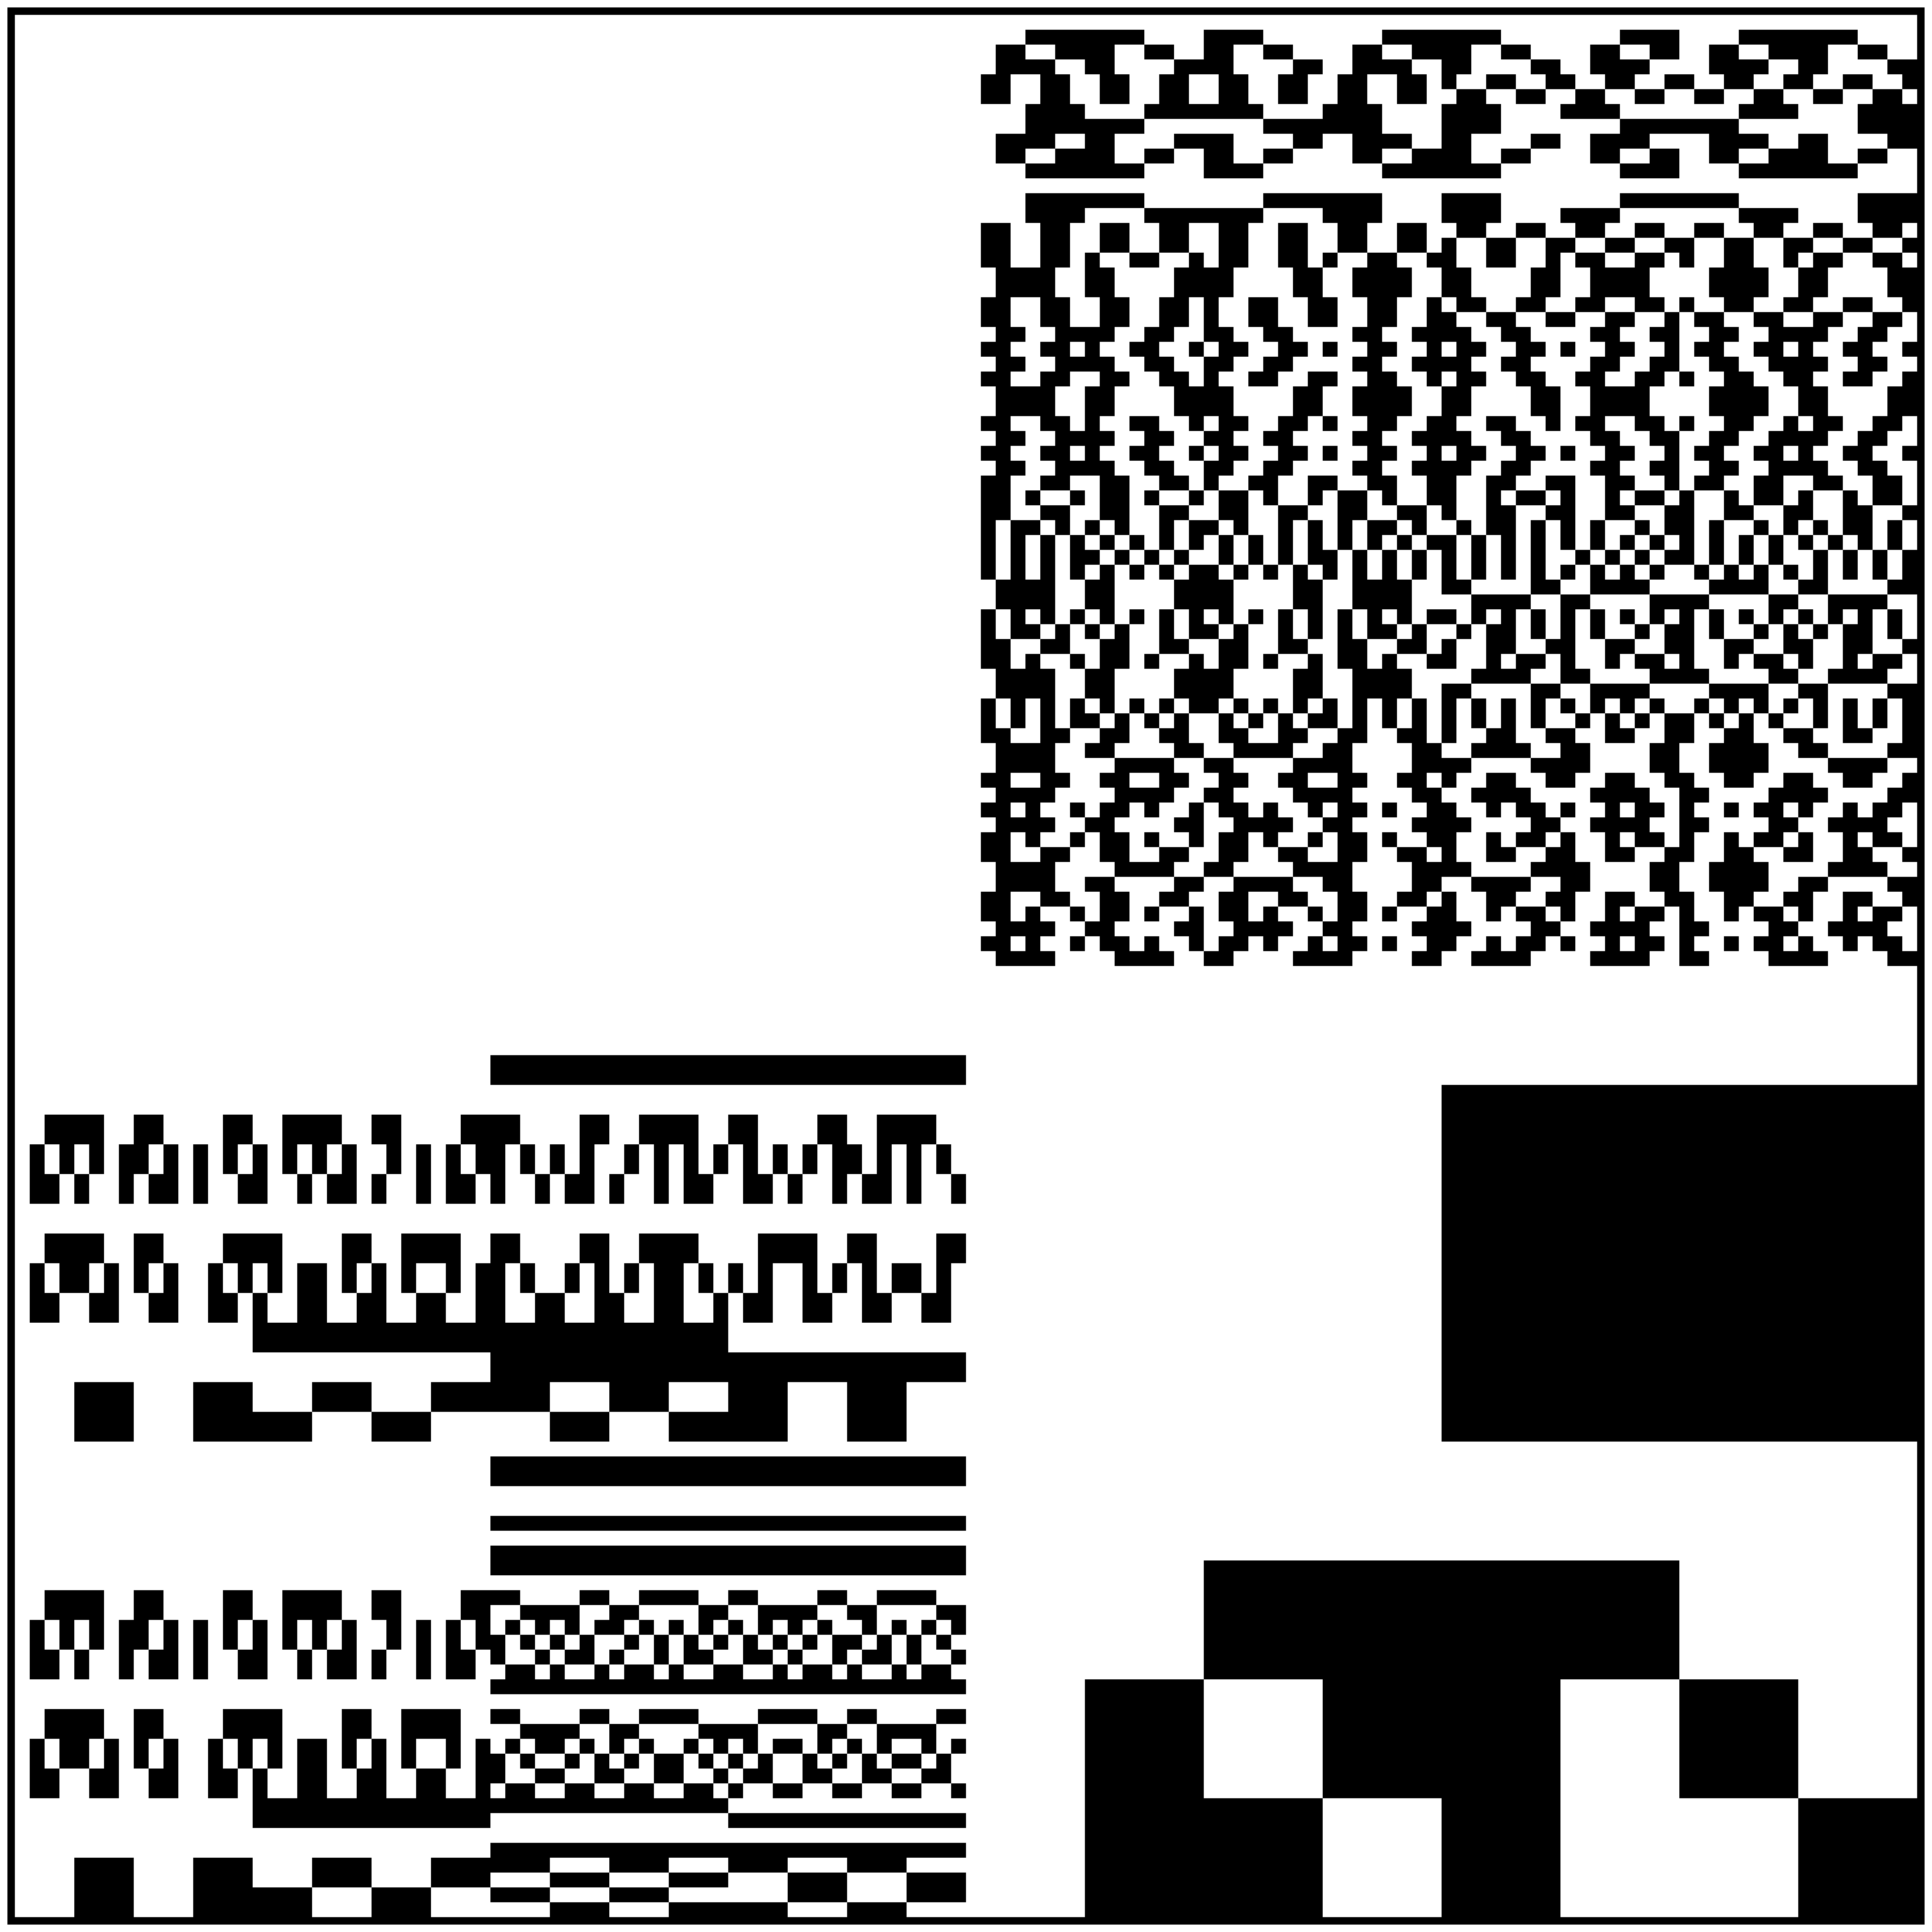
\includegraphics[width=0.8\textwidth]{alpha_awesum.png}
\end{center}
\caption{The restriction of the Parker loop code cocycle $\theta$ to $(V\sqcup W)^2$}
\end{figure}

Remarkably, the restriction of the Parker loop $\cP$ to $V\subset \cG$ reduces to a direct product: $\theta\big|_{V\times V}$ is identically zero! Moreover, the restriction of $\cP$ to $W$ is the direct product $\FF_2^3 \times M$, where $M$ is the Moufang loop from Example~\ref{example:m16}.

% \section{The Golay code and the Parker loop.}

% The extended Golay code $\cG$ is a remarkable object \cite{Thompson}, but here we will be content to give a definition. 
% We shall simply call $\cG$ the `Golay code', since we will not use the 11-dimensional code that is the (unextended) Golay code.
% There is a more-or-less standard basis for $\cG$---using the complement of the adjacency matrix of the icosahedron---but here we shall give a different, very carefully chosen ordered basis.
% And in fact, we shall split the list of basis vectors into two, so as to generate a pair of subspaces $V,W\subset \cG$ to which we will apply Lemma~\ref{lemma:formula lemma}.
% The rows of the left matrix below form the basis for $V$, and the rows of the right matrix below form the basis for $W$.

% \[	
% 	 \left(\begin{array}{c}
%      000110000000010110100011 \\
%      101001111101101111110001 \\
%      000100000000100100111110 \\
%      010000000010000110101101 \\
%      000000000010010101010111 \\
%      100000000000100111110001
%      \end{array}\right)
% \qquad
%     \left(\begin{array}{c}
% 	 101001011100111001111111 \\
% 	 100000011100001001001100 \\
% 	 000001000000111001001110 \\
% 	 100000001000111000111000 \\
% 	 100000000100101000010111 \\
% 	 011011000001111011111111
% 	 \end{array}\right)
% \]






% \[ %%%% Not working, not sure why. LaTeX says "Extra alignment tab has been changed to \cr"
% \begingroup % keep the change local
% \setlength\arraycolsep{2pt}
% \begin{pmatrix}
% 0 & 0 & 0 & 1 & 1 & 0 & 0 & 0 & 0 & 0 & 0 & 0 & 0 & 1 & 0 & 1 & 1 & 0 & 1 & 0 & 0 & 0 & 1 & 1 \\
% 1 & 0 & 1 & 0 & 0 & 1 & 1 & 1 & 1 & 1 & 0 & 1 & 1 & 0 & 1 & 1 & 1 & 1 & 1 & 1 & 0 & 0 & 0 & 1 \\
% 0 & 0 & 0 & 1 & 0 & 0 & 0 & 0 & 0 & 0 & 0 & 0 & 1 & 0 & 0 & 1 & 0 & 0 & 1 & 1 & 1 & 1 & 1 & 0 \\
% 0 & 1 & 0 & 0 & 0 & 0 & 0 & 0 & 0 & 0 & 1 & 0 & 0 & 0 & 0 & 1 & 1 & 0 & 1 & 0 & 1 & 1 & 0 & 1 \\
% 0 & 0 & 0 & 0 & 0 & 0 & 0 & 0 & 0 & 0 & 1 & 0 & 0 & 1 & 0 & 1 & 0 & 1 & 0 & 1 & 0 & 1 & 1 & 1 \\
% 1 & 0 & 0 & 0 & 0 & 0 & 0 & 0 & 0 & 0 & 0 & 0 & 1 & 0 & 0 & 1 & 1 & 1 & 1 & 1 & 0 & 0 & 0 & 1
% \end{pmatrix} 
% \endgroup
% \]

% \section{Graphics.}

% Figures for the \textsc{Monthly} can be submitted as either color or black \& white graphics.  Generally, color graphics will be used for the online publication, and converted to black \& white images for the print journal.  We recommend using whatever graphics program you are most comfortable with, so long as the submitted graphic is provided as a separate file using a standard file format.

% For best results, please follow the following guidelines:
% \begin{enumerate}
% \item Bitmapped file formats---preferably TIFF or JPEG, but not BMP---are appropriate for photographs, using a resolution of at least 300 dpi at the final scaled size of the image.
% \item Line art will reproduce best if provided in vector form, preferably EPS.
% \item Alternatively, both photographs and line art can be provided as PDF files.  Note that creating a PDF does not affect whether the graphic is a bitmap or vector; saving a scanned piece of line art as PDF does not convert it to scalable line art.
% \item If you generating graphics using a \TeX\ package, please be sure to provide a PDF of the manuscript.  In the production process, \TeX-generated graphics will eventually be converted to more conventional graphics so the \textsc{Monthly} can be delivered in e-reader formats.
% \item For photos of contributing authors, we prefer photos that are not cropped tight to the author's profile, so that production staff can crop the head shot to an equal height and width.  If possible, avoid photographs that have excess shadows or glare.
% \end{enumerate}

% \section{Theorems, definitions, proofs, and all that.}

% Following the defaults of the \texttt{amsthm} package, styling is provided for \texttt{theorem}, \texttt{definition}, and \texttt{remark} styles, although the latter two use the same styling.

% \begin{theorem}[Pythagorean Theorem]
% Theorems, lemmas, axioms, and the like are stylized using italicized text. These environments can be numbered or unnumbered, at the author's discretion.
% \end{theorem}

% \begin{proof}
% Proofs set in roman (upright) text, and conclude with an ``end of proof'' (q.e.d.) symbol that is set automatically when you end the proof environment.  When the proof ends with an equation or other non-text element, you need to add \verb~\qedhere~ to the element to set the end of proof symbol; see the \texttt{amsthm} package documentation for more details.
% \end{proof}

% \begin{definition}[Secant Line]
% Definitions, remarks, and notation are stylized as roman text.  They are typically unnumbered, but there are no hard-and-fast rules about numbering.
% \end{definition}

% \begin{remark}
% Remarks stylize the same as definitions.
% \end{remark}


\begin{acknowledgment}{Acknowledgment.}
DMR is supported by the Australian Research Council's Discovery Projects scheme, (project number DP180100383), funded by the Australian Government. \textbf{ADD MORE HERE, IF NEEDED}
\end{acknowledgment}

\begin{thebibliography}{1}

\bibitem{Conway} John H.\ Conway, A simple construction for the Fischer--Griess monster group \emph{Invent.\ math.} \textbf{79} (1985) 513--540.

\bibitem{Griess} Robert L.\ Griess Jr., Code loops \emph{J.\ Algebra} \textbf{100} (1986) 224--234.

\bibitem{Moufang} Moufang, R. (1935), ``Zur Struktur von Alternativk\"orpern'', Math. Ann., 110: 416–430, doi:10.1007/bf01448037

\bibitem{RN_GH} Ben Nagy and David Michael Roberts, \texttt{codeloops}, GitHub repository, (2019) \url{https://github.com/bnagy/codeloops}

\bibitem{Thompson} Thomas M.\ Thompson (1983). From Error Correcting Codes through Sphere Packings to Simple Groups. Carus Mathematical Monographs. \textbf{21}. Mathematical Association of America. 

\end{thebibliography}

\begin{biog}
\item[Ben Nagy] is an MPhil.\ candidate at the University of Adelaide, researching computational stylistics for Latin Poetry.
\begin{affil}
Department of Classics, Archaeology \& Ancient History, The University of Adelaide\\
benjamin.nagy@adelaide.edu.au
\end{affil}

\item[David Michael Roberts] is a mathematician specialising in category theory, geometry and a hodge-podge of other random topics.
\begin{affil}
School of Mathematical Sciences, The University of Adelaide\\
david.roberts@adelaide.edu.au
\end{affil}
\end{biog}
\vfill\eject

\end{document}